\subsection{Recap: Runtime Variability}
\begin{frame}{\insertsubsection}
	\leftorright{
		Basic principles
		\mynote{Runtime parameters}{
			\begin{itemize}
				\item Conditional statements controlled by configuration parameters
				\item Global variables vs. method parameter passing
			\end{itemize}	
		}
		\mynote{Object-oriented concepts and Design Patterns}{
			\begin{itemize}
				\item Template Method
				\item Abstract Factory
				\item Decorator
				\item etc.
			\end{itemize}	
		}
	}{
Problems

Configuration parameters:
Code scattering, tangling, and replication.
	
Design patterns
Trade-offs and potential negative side effects.
Constraints that may restrict their usage.
	
More generally: 
Not well-suited for compile-time binding. 
Variable parts are always delivered.
	}
\end{frame}

\begin{frame}[fragile]{A Basic Graph Implementation}
	\vspace{-1.5cm}
	\begin{flushright}
		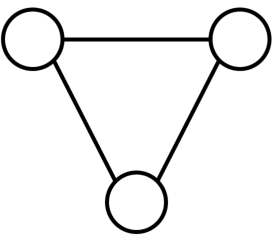
\includegraphics[scale=0.5]{graph-basic}
	\end{flushright}
	\vspace{0.1cm}
	\begin{tiny}
		\begin{columns}
			\column{.45\textwidth}
\begin{lstlisting}
public class Graph {
	List nodes = new ArrayList();
	List edges = new ArrayList();

	Edge add(Node n, Node m) {
		Edge e = new Edge(n, m);
		nodes.add(n); nodes.add(m); edges.add(e);
		return e;
	}
	void print() {
		for (int i = 0; i < edges.size(); i++) {
			((Edge) edges.get(i)).print();
		}
	}
}
\end{lstlisting}
			\column{.45\textwidth}
\begin{lstlisting}
public class Node {
	int id = 0;

	void print() {
		System.out.print(id);
	}
}
\end{lstlisting}
\begin{lstlisting}
public class Edge {
	Node a, b;

	Edge(Node _a, Node _b) {
		a = _a; b = _b;
	}
	void print() {
		a.print(); b.print();
	}
}
\end{lstlisting}
		\end{columns}
	\end{tiny}
\end{frame}

\begin{frame}[fragile]{Evolution Step: Weighted Graphs}
	\vspace{-1.5cm}
	\begin{flushright}
		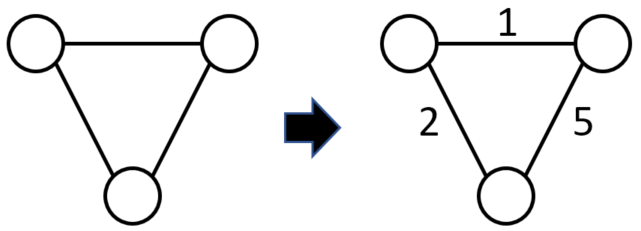
\includegraphics[scale=0.5]{graph-basic-to-weighted}
	\end{flushright}
	\vspace{0.1cm}
	\begin{tiny}
		\begin{columns}
			\column{.45\textwidth}
\begin{lstlisting}
public class Graph {
	List nodes = new ArrayList();
	List edges = new ArrayList();

	Edge add(Node n, Node m) {
		Edge e = new Edge(n, m);
		nodes.add(n); nodes.add(m); edges.add(e);
		@e.weight = new Weight();@
		return e;
	}
	@Edge add(Node n, Node m, Weight w) {
		Edge e = new Edge(n, m);
		nodes.add(n); nodes.add(m); edges.add(e);
		e.weight = w;
		return e;
	}@
	void print() {
		for (int i = 0; i < edges.size(); i++) {
			((Edge) edges.get(i)).print();
		}
	}
}
\end{lstlisting}
			\column{.45\textwidth}
\begin{lstlisting}
public class Edge {
	Node a, b;
	@Weight weight = new Weight();@

	Edge(Node _a, Node _b) {
		a = _a; b = _b;
	}
	void print() {
		a.print(); b.print();
		@weight.print();@
	}
}
\end{lstlisting}
\begin{lstlisting}
@public class Weight {
	void print() {...}
}@
\end{lstlisting}
		\end{columns}
	\end{tiny}
\end{frame}

\begin{frame}[fragile]{Evolution Step: Colored Graphs}
	\vspace{-1.5cm}
	\begin{flushright}
		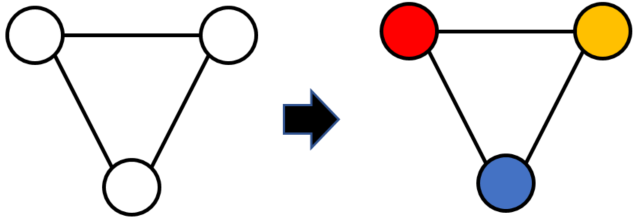
\includegraphics[scale=0.5]{graph-basic-to-colored}
	\end{flushright}
	\vspace{0.1cm}
	\begin{tiny}
		\begin{columns}
			\column{.45\textwidth}
\begin{lstlisting}
public class Graph {
	List nodes = new ArrayList();
	List edges = new ArrayList();

	Edge add(Node n, Node m) {
		Edge e = new Edge(n, m);
		nodes.add(n); nodes.add(m); edges.add(e);
		return e;
	}
	void print() {
		for (int i = 0; i < edges.size(); i++) {
			((Edge) edges.get(i)).print();
		}
	}
}
\end{lstlisting}	
			\column{.45\textwidth}
\begin{lstlisting}
public class Node {
	int id = 0;
	~Color color = new Color();~

	void print() {
		~Color.setDisplayColor(color);~
		System.out.print(id);
	}
}
\end{lstlisting}
\begin{lstlisting}
~public class Color {
	static void setDisplayColor(Color c) {...}
}~
\end{lstlisting}
		\end{columns}
	\end{tiny}
\end{frame}

\begin{frame}{Problem: Dealing With New Requirements}
	\leftorright{
		\myexample{New requirement}{
			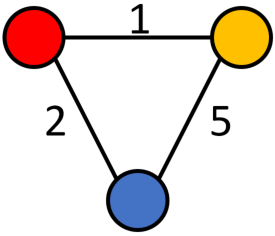
\includegraphics[scale=0.4]{graph-weighted-colored}
		}
	}{
		\myexample{Where to start from?}{
			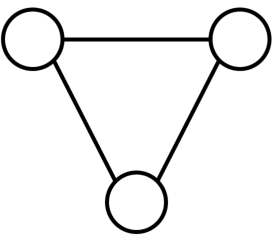
\includegraphics[scale=0.4]{graph-basic}
			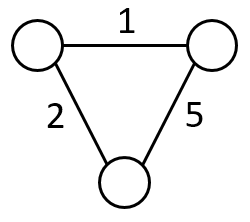
\includegraphics[scale=0.4]{graph-weighted}
			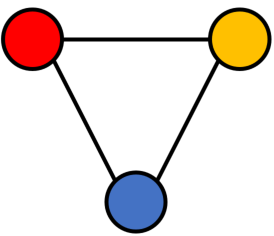
\includegraphics[scale=0.4]{graph-colored}
		}
	}
\end{frame}

\begin{frame}[fragile]{Problem: Evolution and Maintenance}
	\begin{columns}
		\column{.15\textwidth}
			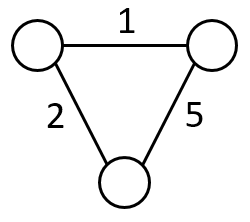
\includegraphics[width=\linewidth]{graph-weighted}
		\column{.3\textwidth}
\begin{tiny}
\begin{lstlisting}
public class Graph {
	...
	Edge add(Node n, Node m) {
		Edge e = new Edge(n, m);
		nodes.add(n); nodes.add(m); edges.add(e);
		@e.weight = new Weight();@
		return e;
	}
	@Edge add(Node n, Node m, Weight w) {
		Edge e = new Edge(n, m);
		nodes.add(n); nodes.add(m); edges.add(e);
		e.weight = w;
		return e;
	}@
	...
}
\end{lstlisting}
\end{tiny}
		\column{.025\textwidth}
			\begin{LARGE}
				$\Rightarrow$
			\end{LARGE}
		\column{.3\textwidth}
\begin{tiny}
\begin{lstlisting}
public class Graph {
	...
	Edge add(Node n, Node m) {
		Edge e = new Edge(n, m);
		nodes.add(n); nodes.add(m); edges.add(e);
		@e.weight = new Weight();@
		return e;
	}
	@Edge add(Node n, Node m, Weight w) {
		Edge e = this(n, m);
		e.weight = w;
		return e;
	}@
	...
}
\end{lstlisting}
\end{tiny}
	\end{columns}
	\myexample{Where and how to propagate the improvement (here: refactoring)}{
		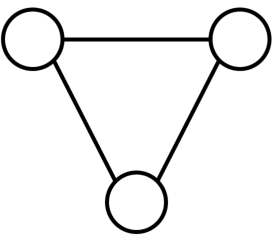
\includegraphics[scale=0.4]{graph-basic}
		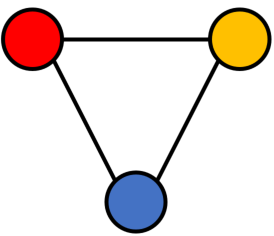
\includegraphics[scale=0.4]{graph-colored}
		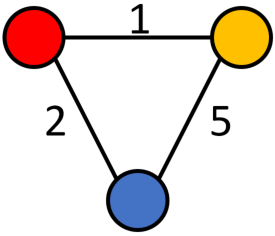
\includegraphics[scale=0.4]{graph-weighted-colored}
	}
\end{frame}